\section{Ablation}\label{sec:ablation}

\subsection{Variants and what each removes}

The ablation removes one component of the sequence at a time on the acceptance task at \parFrames{} frames over \ablTN{} seeds, with the same seeds as the main result. The variants are: the sequence with all components; the sequence without the trajectory lock, in which the phase of each coefficient is the phase of the current field as in the induced sequence, while the weights are still carried across frames and the positions still follow the minimal-jerk profile; the sequence without the per-frame optimization, in which every frame is the inverse transform of the prescribed spots with unit weights and no iteration, so that only the lock and the profile remain; the sequence with 1 and with 3 iterations per frame instead of \parFrameIters{}; and the sequence with a linear time profile for the positions instead of the minimal-jerk profile, with the same frame count. The two published sequences are reproduced from Table~\ref{tab:main} as references. Table~\ref{tab:ablation} gives the results and Fig.~\ref{fig:ablation} shows them per seed. The variant with all components is checked against the module of the engine and agrees to \ablTCheck{}, so the other rows are the module with parts removed.

\begin{table}[t]
\centering\small
\caption{Ablation of the flicker-bounded sequence on the acceptance task at \parFrames{} frames over \ablTN{} seeds: transient minimum ratio (mean $\pm$ standard deviation, range), seeds at $0.9$ or above, largest per-frame spread and largest phase step (medians over the seeds); the three last rows are the published sequences for reference.}
\label{tab:ablation}
\adjustbox{max width=\textwidth}{\begin{tabular}{@{}l r r r r r@{}}
\toprule
Variant & Minimum ratio, mean $\pm$ s.d. & Range & Seeds at 0.9 or above & Largest frame $\sigma$ (\%) & Largest phase step (rad) \\
\midrule
flicker-bounded sequence, all components & 0.923 $\pm$ 0.007 & 0.915 to 0.932 & 6 of 6 & 0.24 & 0.069 \\
without the trajectory lock & 0.884 $\pm$ 0.055 & 0.776 to 0.924 & 4 of 6 & 2.45 & 0.455 \\
without the per-frame optimization & 0.789 $\pm$ 0.038 & 0.724 to 0.830 & 0 of 6 & 17.67 & 0.064 \\
1 iteration per frame & 0.747 $\pm$ 0.069 & 0.676 to 0.823 & 0 of 6 & 18.62 & 0.063 \\
3 iterations per frame & 0.918 $\pm$ 0.010 & 0.905 to 0.933 & 6 of 6 & 3.50 & 0.066 \\
linear time profile for the positions & 0.967 $\pm$ 0.006 & 0.959 to 0.974 & 6 of 6 & 0.21 & 0.041 \\
linear phase interpolation (reference) & 0.644 $\pm$ 0.057 & 0.551 to 0.709 & 0 of 6 & 23.50 & 0.409 \\
per-frame GS with phase induction, 5 iterations (reference) & 0.948 $\pm$ 0.017 & 0.918 to 0.965 & 6 of 6 & 2.23 & 0.302 \\
per-frame GS with phase induction, 10 iterations (reference) & 0.925 $\pm$ 0.034 & 0.880 to 0.966 & 4 of 6 & 1.29 & 0.499 \\
\bottomrule
\end{tabular}
}
\end{table}

\begin{figure}[t]
\centering
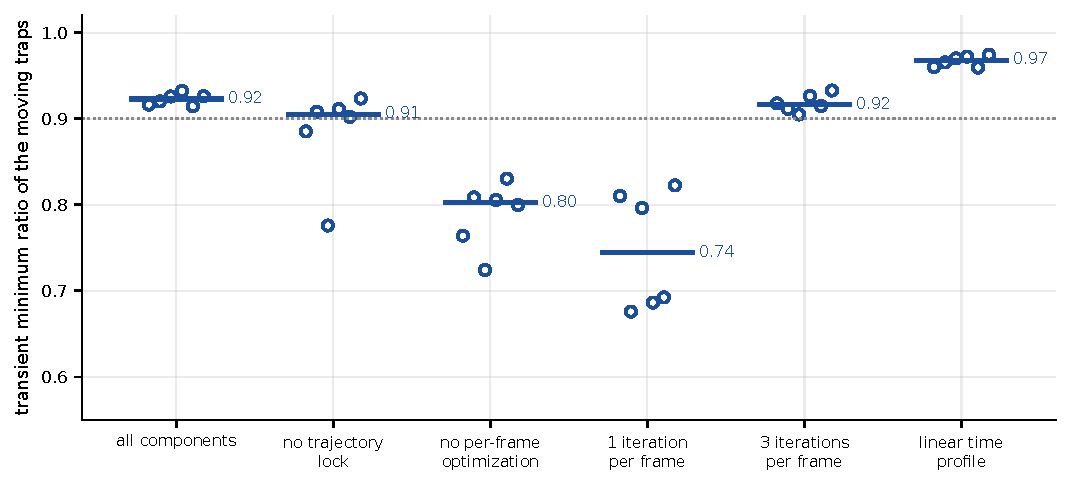
\includegraphics[width=\textwidth]{fig-ablation.pdf}
\caption{Transient minimum ratio of the moving traps per seed for the full sequence and each ablated variant on the acceptance task; markers are seeds, bars are medians, and the dotted line is $0.9$. Removing the per-frame optimization or reducing the iterations to one puts every seed below $0.9$; removing the lock spreads the seeds widely; the linear time profile raises every seed.}
\label{fig:ablation}
\end{figure}

\subsection{Reading the ablation}

\emph{The per-frame optimization is necessary.} Without it the mean falls from \ablTFullMean{} to \ablTNoOptMean{} (standard deviation \ablTNoOptSd{}), no seed reaches $0.9$, and the largest per-frame spread rises from \ablTFullSig{} to \ablTNoOptSig{} percent, close to the \accLpiSigmaMed{} percent of linear phase interpolation. The phase step stays small, \ablTNoOptStep{} rad, since the lock still holds. The variant is better than linear phase interpolation, \accLpiTransMean{}, so the locked phases explain part of the gap to it, and the optimization explains the rest. H7 held.

\emph{The lock does not move the mean as far as the optimization, but it controls the step and the spread of outcomes.} Without the lock the mean is \ablTNoLockMean{} (standard deviation \ablTNoLockSd{}, range \ablTNoLockMin{} to \ablTNoLockMax{}) against \ablTFullMean{} (\ablTFullSd{}), and a majority of seeds still reaches $0.9$, so H6 is refuted by the rule fixed in advance. What changes is the phase step, from \ablTFullStep{} to \ablTNoLockStep{} rad, a factor of \lockStepRatio{}, and the largest spread of a frame, from \ablTFullSig{} to \ablTNoLockSig{} percent. The unlocked variant has the phase step of the induced sequences: \ablTNoLockStep{} rad against the median of \accKimTenStepMed{} rad for the per-frame method at the same iteration count. This is the evidence that the lock, and not the carried weights or the profile, is what reduces the step, and it is the consistency check of Proposition~\ref{prop:lock}.

\emph{Three iterations suffice.} With 3 iterations per frame the mean is \ablTItersThreeMean{}, indistinguishable from \ablTFullMean{} at ten, while with one iteration it falls to \ablTItersOneMean{}. The iteration count of the main experiments, \parFrameIters{}, is therefore conservative for this task, and a sequence with 3 iterations per frame does less work than the per-frame method at \parKimIters{} iterations while reaching a similar level, \ablTItersThreeMean{} against \accKimFiveTransMean{}. Because the experiments of the paper use \parFrameIters{} for the proposed sequence, the comparison with the per-frame method at 5 iterations is in fact favourable to the per-frame method on work, and the comparison at \parFrameIters{} is the equal-work one.

\emph{The minimal-jerk profile lowers the transient minimum on this task.} With a linear time profile and the same number of frames the mean rises to \ablTLinearMean{} (range \ablTLinearMin{} to \ablTLinearMax{}), above the per-frame method at \parKimIters{} iterations by \linearGap{} in the mean, and the median of the largest phase step is \ablTLinearStep{} rad. Table~\ref{tab:profile} reads this variant by the benchmark rule against every baseline: it is better on the dip and on the spread than the per-frame method at both iteration counts and than linear phase interpolation. The reason is Proposition~\ref{prop:frames}: the minimal-jerk profile has a peak velocity of $15/8$ times the mean, so at the same frame count its peak shift between frames is almost twice that of the linear profile, and the transient ratio depends on the peak shift. The minimal-jerk profile is the default for a reason that concerns the motion of atoms and that the cited experiment supports only for a different system (Section~\ref{sec:flicker-method}); the hologram measurements here do not weigh that reason, and they score the linear profile higher on every measure of the table.

Taken together, the ablation says that the value of the sequence lies in the combination of the lock with the per-frame optimization, that the lock is what lowers the phase step, that three iterations per frame suffice on this task, and that the time profile is a parameter that decides the reading against the published per-frame method: the default minimal-jerk profile loses the dip to it at the frame count of the acceptance task, and the linear profile wins. These are the conclusions that Section~\ref{sec:discussion} draws on.
